\documentclass[a4paper,11pt]{report}
\usepackage[T1]{fontenc}
\usepackage[utf8]{inputenc}
\usepackage{lmodern}
\usepackage[francais]{babel}
\usepackage{graphicx,color,caption2}
\usepackage{epsfig}
\usepackage{fancyhdr}
%\usepackage{fancyvrb}
\usepackage{textcomp}
\pagestyle{fancy}
\usepackage{listings} % pour incorporer des sources
\usepackage{listingsutf8} % pour incorporer des sources
\usepackage[francais]{layout} % pour obtenir le layout
\usepackage{fullpage} % pour obtenir le layout
\usepackage{makeidx} % pour créer une table d'index
%\usepackage{shadow} % pour faire des encadrements
\oddsidemargin -4mm % Marge de gauche -4mm
\textwidth 17cm % Largeur de gauche = 17cm
\textheight 22cm % Hauteur du texte = 22cm
\parindent 0cm % Pas d'indentation de paragraphe
\lstset{language={},%C,Assembleur, TeX, tcl, basic, cobol, fortran, logo, make, pascal, perl, prolog, {}
literate={â}{{\^a}}1 {ê}{{\^e}}1 {î}{{\^i}}1 {ô}{{\^o}}1 {û}{{\^u}}1
{ä}{{\"a}}1 {ë}{{\"e}}1 {ï}{{\"i}}1 {ö}{{\"o}}1 {ü}{{\"u}}1
{à}{{\`a}}1 {é}{{\'e}}1 {è}{{\`e}}1 {ù}{{\`u}}1
{Â}{{\^A}}1 {Ê}{{\^E}}1 {Î}{{\^I}}1 {Ô}{{\^O}}1 {Û}{{\^U}}1
{Ä}{{\"A}}1 {Ë}{{\"E}}1 {Ï}{{\"I}}1 {Ö}{{\"O}}1 {Ü}{{\"U}}1
{À}{{\`A}}1 {É}{{\'E}}1 {È}{{\`E}}1 {Ù}{{\`U}}1,
commentstyle=\scriptsize\ttfamily\slshape, % style des commentaires
basicstyle=\scriptsize\ttfamily, % style par défaut
keywordstyle=\scriptsize\rmfamily\bfseries,% style des mots-clés
backgroundcolor=\color[rgb]{.95,.95,.95}, % couleur de fond : gris clair
framerule=0.5pt,% Taille des bords
frame=trbl,% Style du cadre
frameround=tttt, % Bords arrondis
tabsize=3, % Taille des tabulations
% extendedchars=\true, % Incompatible avec utf8 et literate
inputencoding=utf8,
showspaces=false, % Ne montre pas les espaces
showstringspaces=false, % Ne montre pas les espaces entre '
xrightmargin=0.5cm, % Retrait gauche
xleftmargin=0.5cm, % Retrait droit
escapechar=@}  % Caractère d'échappement, permet des commandes latex dans la source


\title{Client / server}
\author{Akachar Yassine}

\begin{document}

\maketitle
\tableofcontents
\chapter{
  \title{Introduction}
}
\section{Librairie socket}
L'objectif de ce travail est de créer une application client/serveur afin que plusieurs utilisateurs puissent se connecter et y stocker toutes sortes d'informations.
Pour ce faire, il faudra lancer un serveur sur une machine, et au minimum un client sur une autre machine. Pour ce travail, c'est par la librairie socket que l'on passe pour permettre cette connexion.


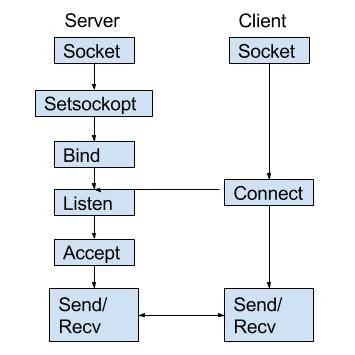
\includegraphics[width=115mm]{./resources/socket.jpg}

\section{Appel system fork}
Pour pouvoir assurer la connection avec plusieurs utilisateurs simultanement, on utilise l'appel system fork. De ce fait, nous allons pouvoir dupliquer autant de fois le process qu'il n'y a d'utilisateurs et ainsi leur permettre d'agir "en même temps" tout en ayant un seul et unique serveur.

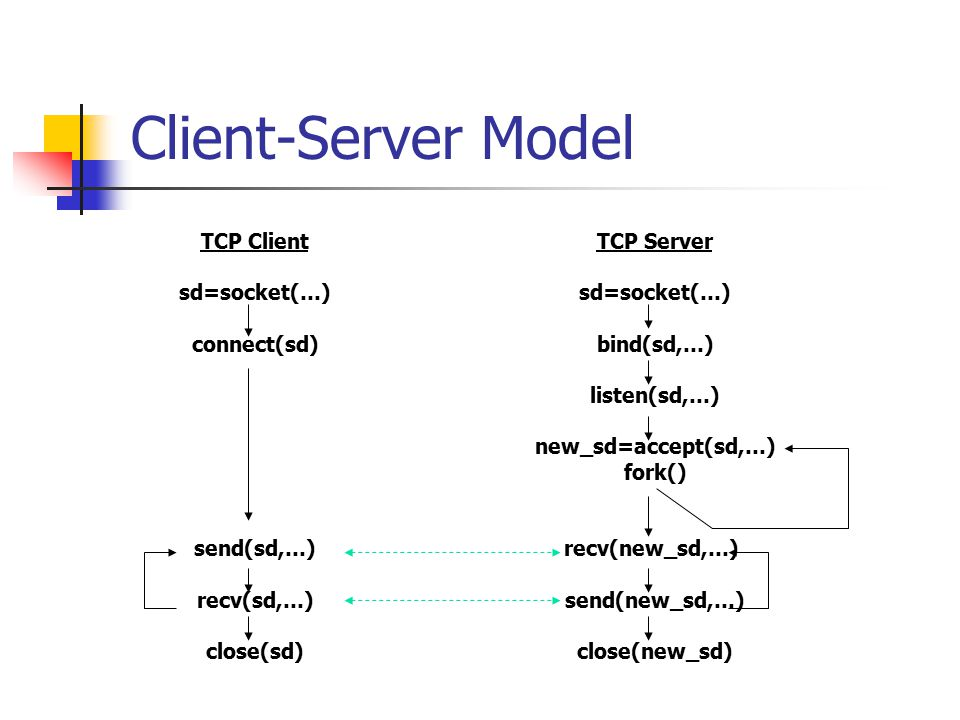
\includegraphics[width=115mm]{./resources/socketFork.jpg}

\subsection{Comment ca marche ?}
L'appel système fork retorune une valeur entière. Pour pouvoir différencier le processus pere du fils il faut regarder la valeur du fork. Si cette valeur est nulle, c'est que nous sommes dans le processus fils, sinon la valeur est égale au pid du fils au quel cas nous sommes dans le processus père.


\begin{lstlisting} 
    int main(void)
{
  printf("processus pere, avant le fork\n");
  int pid = fork();
  if (pid == 0)
    printf("processus fils, apres le fork\n");
  else
    printf("processus pere, apres le fork (pid du fils = %d)\n", pid);
  printf("fin de processus\n");
}
\end{lstlisting}
Ce qui donne :
\begin{lstlisting} 
processus pere, avant le fork
processus fils, apres le fork
processus pere, apres le fork (pid du fils = 25532)
fin de processus
fin de processus
\end{lstlisting}

    
\chapter{Serveur}
\textbf{} 
\section{Code source}
\lstinputlisting[inputencoding=utf8/latin1]{./SYSG5-Proj/serverFork.c}
\subsection{Variables}
\begin{itemize}
            \item $serverAddr$ : représente la structure sockaddr\_in contenant les informations du serveur
            \item $newAddr$ : représente la structure sockaddr\_in qui contiendra les informations de chaque client (une variable pour chaque client)
            \item $sockfd$ : représente le socket à qui l'on va assigné l'adresse du serveur grâce à la structure sockaddr\_in
            \begin{lstlisting} 
                ret = bind(sockfd, &serverAddr, sizeof(serverAddr));
            \end{lstlisting}
            \item $newSocket$ : représentera le socket qui permettra l'échange entre le serveur et le client
            \begin{lstlisting} 
                newSocket = accept(sockfd, (struct sockaddr*)&newAddr, &addr_size);
            \end{lstlisting}
\end{itemize}
\subsection{Fork}
Concentrons nous sur la partie duplication de process. Grâce au l'appel systeme fork, nous pouvons dupliquer autant de fois notre process ce qui nous permet d'avoir autant de client que nous voulons. Cependant, pour ne pas surcharger le serveur et empêcher que trop de personnes se connectent au serveur et le fasse crasher, nous allons limiter le nombre de client connecté en même temps. Nous allons le spécifier lors de l'appel à la fonction listen. La fonction listen() marque le socket spécifié comme un socket passive, c'est à dire un socket prêt à accepter les demandes de connections (fonction accept citée au dessus).
\begin{lstlisting} 
      listen(sockfd, 10)
\end{lstlisting}


Une fois le socket passif, et une connexion acceptée, Il faut pouvoir gérer la connexion de chaque client individuellement tout en maintent le serveur actif. 
D'où la duplication de process. 
Comme expliqué précédemment, en vérifiant que le retour de l'appel systeme fork soit égale à 0, on sait que tout ce qui est exécutés entre accolade du if ne sera exécutés que par le processus fils.
\begin{lstlisting} 
     if((childpid = fork()) == 0){
          ...
     }
\end{lstlisting}


\chapter{Client}
\section{Code source}
\lstinputlisting[inputencoding=utf8/latin1]{./SYSG5-Proj/clientFork.c}
\subsection{Variables}
\begin{itemize}
            \item $serverAddr$ : représente la structure sockaddr\_in contenant les informations du serveur
            \item $clientSocket$ : représente le socket que l'on va connecter à l'adresse dur serveur et qui nous permettra l'échange avec le serveur            
            
\end{itemize}
\subsection{Connection}
Une fois le socket créé, il faut le connecter. Cela se fait grâce à la fonction connect.
\begin{lstlisting} 
     ret = connect(clientSocket, &serverAddr, sizeof(serverAddr));
	  if(ret == -1){
		  perror("[-]Error in connection.\n");
		exit(1);
	}
\end{lstlisting}
	Si connect retourne -1, c'est que la connection à échouer. Grâce à perror, on peut en savoir la cause exact.
\subsection{Commandes}

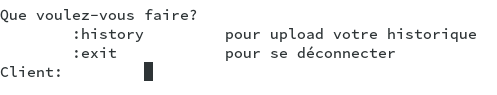
\includegraphics[width=115mm]{./resources/commandes.png}

\begin{enumerate}
  \item :history permet d'envoyer son historique
  \item :exit permet de se seconnecter
\end{enumerate}

\subsection{client.sh}

C'est un script qui charge les n dernières commandes tapés par le client et lancer le client. 
\lstinputlisting[inputencoding=utf8/latin1]{./SYSG5-Proj/client.sh}

\chapter{Configuration}

\section{Coté serveur}
Avant de lancer le serveur, il faut s'assurer que le firewall est désactivé. S'il ne l'est pas , impossible de joindre le serveur puisqu'il ne laissera rien passer.
\begin{lstlisting} 
   sudo rcSuSEfirewall2 stop // pour executer en tant qu'administrateur
\end{lstlisting}
Pour le serveur, c'est tout ce qu'il faut faire.
Une fois le firewall désactivé, vous pouvez compiler le fichier serverfork.c lancer votre serveur de la sorte 
\begin{lstlisting} 
gcc -w -Wall -o server serverFork.c
./server XXX.XXX.XXX.XXX   //où XXX.XXX.XXX.XXX est l'adresse du serveur.
\end{lstlisting}




\section{Coté client}
Avant de lancer le client, il faut s'assurer que l'historique de commande se met à jour à chaque fois qu'une commande est entrée. Il faut copier ses deux lignes dans le fichiers ~/.bashrc. Ensuite redémarrer pour mettre à jour les modifications.
\begin{lstlisting} 
shopt -s histappend                      # active la fonction append pour l'historique
export PROMPT_COMMAND="history -a; history -c; history -r; $PROMPT_COMMAND"
\end{lstlisting}
Une fois le fichier ~/.bashrc à jour, vous devez modifier dans le script client.sh et y mettre l'adresse à laquelle vous voulez vous connecter et entrer l'adresse de votre serveur 

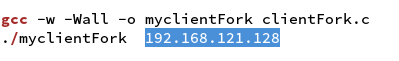
\includegraphics[width=100mm]{./resources/adresseServeur.png}

\end{document}
